\documentclass{article}

\usepackage[preprint]{neurips_2025}

\usepackage[utf8]{inputenc}
\usepackage[T1]{fontenc}
\usepackage{hyperref}
\usepackage{url}
\usepackage{booktabs}
\usepackage{amsfonts}
\usepackage{amsmath}
\usepackage{microtype}
\usepackage{xcolor}
\usepackage[skip=3pt,font=small]{caption}
\usepackage{graphicx}

\graphicspath{{../artifacts/figures/}}

% Let floats take more of a page so tables do not get deferred past the text.
\renewcommand{\topfraction}{0.92}
\renewcommand{\bottomfraction}{0.85}
\renewcommand{\textfraction}{0.06}
\renewcommand{\floatpagefraction}{0.80}
\setlength{\textfloatsep}{10pt plus 2pt minus 2pt}
\setlength{\intextsep}{10pt plus 2pt minus 2pt}

% Measured quantities are generated by src/figures.py so no number is typed by hand.
\providecommand{\distilParams}{}\renewcommand{\distilParams}{67.0}
\providecommand{\bertParams}{}\renewcommand{\bertParams}{110.1}
\providecommand{\paramReduction}{}\renewcommand{\paramReduction}{39}
\providecommand{\gpuLatencyDistil}{}\renewcommand{\gpuLatencyDistil}{2.57}
\providecommand{\gpuLatencyBert}{}\renewcommand{\gpuLatencyBert}{4.25}
\providecommand{\gpuSpeedup}{}\renewcommand{\gpuSpeedup}{1.65}
\providecommand{\cpuLatencyDistil}{}\renewcommand{\cpuLatencyDistil}{34.5}
\providecommand{\cpuLatencyBert}{}\renewcommand{\cpuLatencyBert}{62.7}
\providecommand{\cpuSpeedup}{}\renewcommand{\cpuSpeedup}{1.82}
\providecommand{\throughputDistil}{}\renewcommand{\throughputDistil}{1830}
\providecommand{\throughputBert}{}\renewcommand{\throughputBert}{914}
\providecommand{\throughputSpeedup}{}\renewcommand{\throughputSpeedup}{2.00}
\providecommand{\trainMemDistil}{}\renewcommand{\trainMemDistil}{1.48}
\providecommand{\trainMemBert}{}\renewcommand{\trainMemBert}{2.64}
\providecommand{\memReduction}{}\renewcommand{\memReduction}{44}
\providecommand{\inferMemDistil}{}\renewcommand{\inferMemDistil}{475}
\providecommand{\inferMemBert}{}\renewcommand{\inferMemBert}{640}
\providecommand{\meanAccDistil}{}\renewcommand{\meanAccDistil}{92.84}
\providecommand{\meanAccBert}{}\renewcommand{\meanAccBert}{93.63}
\providecommand{\meanAccGap}{}\renewcommand{\meanAccGap}{0.78}
\providecommand{\meanFoneDistil}{}\renewcommand{\meanFoneDistil}{92.84}
\providecommand{\meanFoneBert}{}\renewcommand{\meanFoneBert}{93.62}
\providecommand{\meanFoneGap}{}\renewcommand{\meanFoneGap}{0.78}
\providecommand{\accRetention}{}\renewcommand{\accRetention}{99.2}
\providecommand{\maxAccGap}{}\renewcommand{\maxAccGap}{1.61}
\providecommand{\minAccGap}{}\renewcommand{\minAccGap}{-0.04}
\providecommand{\minGapDataset}{}\renewcommand{\minGapDataset}{AG News}
\providecommand{\maxGapDataset}{}\renewcommand{\maxGapDataset}{SST 2}
\providecommand{\nDatasets}{}\renewcommand{\nDatasets}{2}
\providecommand{\nRuns}{}\renewcommand{\nRuns}{4}
\providecommand{\bertWins}{}\renewcommand{\bertWins}{1}
\providecommand{\distilTiesOrWins}{}\renewcommand{\distilTiesOrWins}{1}
\providecommand{\trainMinutesDistil}{}\renewcommand{\trainMinutesDistil}{7}
\providecommand{\trainMinutesBert}{}\renewcommand{\trainMinutesBert}{11}
\providecommand{\wordOverlap}{}\renewcommand{\wordOverlap}{7.3}
\providecommand{\wordOverlapPct}{}\renewcommand{\wordOverlapPct}{73}
\providecommand{\wordCka}{}\renewcommand{\wordCka}{0.898}
\providecommand{\nWords}{}\renewcommand{\nWords}{496}
\providecommand{\purityBert}{}\renewcommand{\purityBert}{69}
\providecommand{\purityDistil}{}\renewcommand{\purityDistil}{72}
\providecommand{\ckaEmbeddings}{}\renewcommand{\ckaEmbeddings}{0.977}
\providecommand{\ckaTop}{}\renewcommand{\ckaTop}{0.578}
\providecommand{\ckaMid}{}\renewcommand{\ckaMid}{0.838}
\providecommand{\ckaMidDistilLayer}{}\renewcommand{\ckaMidDistilLayer}{3}
\providecommand{\ckaMidBertLayer}{}\renewcommand{\ckaMidBertLayer}{6}
\providecommand{\sentCka}{}\renewcommand{\sentCka}{0.880}


\title{DistilBERT and BERT for Text Classification:\\ Performance, Efficiency and the Role of the Classifier Head}

\author{%
  Ricardo Amiel Acu\~na Villogas \quad Juan Leibniz Aquino Espinoza \quad Josu\'e Nehem\'ias Velo Poma \\
  Universidad de Ingenier\'ia y Tecnolog\'ia (UTEC) \\
  \texttt{\{ricardo.acuna, juan.aquino, josue.velo\}@utec.edu.pe}
}

\begin{document}

\maketitle

\begin{abstract}
We present an evaluation of using knowledge distillation to train a smaller encoder DistilBERT from a base BERT as the teacher. We fine tune DistilBERT and BERT base under an identical classifier, optimiser and data budget on \nDatasets{} text classification datasets: AG News, SST 2, Yelp Polarity and Yelp Review Full. DistilBERT holds \paramReduction{} percent fewer parameters and reaches \accRetention{} percent of the accuracy of BERT, a mean gap of \meanAccGap{} points ranging from \minAccGap{} to \maxAccGap{} across datasets, in exchange for \throughputSpeedup{} times the inference throughput and \memReduction{} percent less peak GPU memory in training. A seven way ablation over the classifier shows its shape is almost irrelevant: width and depth move F1 macro by at most \headSpread{} points, while freezing the transformer costs \frozenGap{}. Over \nWords{} words, \wordOverlapPct{} percent of nearest neighbours are shared between the two pretrained encoders, at a linear CKA of \wordCka{}. What distillation gave up is capacity, not the organisation of the space.
\end{abstract}

\section{Introduction}

BERT \citep{devlin2019bert} made pretrained bidirectional transformers \citep{vaswani2017attention} the
default starting point for text classification, at a cost that is awkward in deployment: 110 million
parameters and a twelve block forward pass per input. DistilBERT \citep{sanh2019distilbert} answers with
knowledge distillation \citep{hinton2015distilling}, training a six block student against the teacher
output distribution, its hidden states and the masked language modelling objective, and reports roughly
97 percent of the GLUE score \citep{wang2018glue} of BERT with 40 percent fewer parameters.

This report is a controlled comparison of those two models on text classification. It proposes no method.
It replaces that aggregate headline with the three measurements needed before choosing a backbone for one
task: how large the accuracy gap is on that dataset, what the smaller model buys in latency and memory, and
whether any of the gap can be recovered by spending capacity on the classifier instead of the encoder. Both
backbones get the same classifier, optimiser and data budget, on four datasets, plus an ablation over the
classifier along the three axes a practitioner controls, freezing, width and depth, and a representation
level comparison of the two encoders.

\section{Approach}

\paragraph{What distillation changed.}
DistilBERT keeps the hidden size of 768 and the vocabulary of BERT base, removes every second transformer
block leaving six, and drops the token type embeddings and the pooler. The student is initialised from
alternate teacher layers and trained with three losses: distillation against the softened teacher
distribution, masked language modelling, and a cosine term aligning student and teacher hidden state
directions \citep{sanh2019distilbert}. Depth is the axis that was cut; width, vocabulary and attention are
untouched.

\paragraph{One classifier for both backbones.}
Both backbones are wrapped in the same module. The final hidden state of the \texttt{[CLS]} position,
$h \in \mathbb{R}^{768}$, is passed through an MLP $\hat{y} = W_L\,\sigma(\cdots \sigma(W_1\,
\mathrm{drop}(h)) \cdots)$ with $\sigma = \mathrm{ReLU}$ and dropout before every linear map. We
deliberately do not use the BERT pooler, which DistilBERT does not have, so both models are read the same
way and no architectural advantage enters through pooling. The baseline head is one hidden layer of 768
units, reproducing the default DistilBERT design, and the same head exposes the three ablation axes:
freezing covers the embeddings and the first $n$ blocks, with $n$ equal to all blocks giving a linear
probe; width is the units per hidden layer; depth is the number of hidden layers.

\paragraph{What we measure.}
Accuracy with macro averaged precision, recall and F1 on the test split, macro averaged so the five class
Yelp task is not dominated by its easiest classes; parameter count, single example latency, throughput at
batch 32 and peak GPU memory. Latency is the median of 200 timed float32 passes after 20 warmup passes with
device synchronisation, and memory is read from the CUDA allocator rather than the driver. Training and
validation loss are recorded at twelve equally spaced iterations, the validation loss on a held out slice
of train, so the test split is never touched during optimisation.

\section{Experiments}

\paragraph{Setup.}
AG News is four way topic classification \citep{zhang2015character}; SST 2 is binary sentiment
\citep{socher2013recursive} through GLUE \citep{wang2018glue}, whose labelled validation split serves as the
test set as usual; Yelp Polarity and Yelp Review Full are binary and five star review sentiment
\citep{zhang2015character}, each subsampled to 100{,}000 training and 10{,}000 test examples. Five percent
of every training set is held out for the loss curves. Every run uses AdamW \citep{loshchilov2019adamw} at
$2 \times 10^{-5}$ on the backbone and $10^{-4}$ on the head, weight decay 0.01, linear decay with 6 percent
warmup, batch 32, clipping at 1.0 and bfloat16 autocast, with maximum length 64 for SST 2, 128 for AG News
and 256 for Yelp. Two epochs sits inside the fine tuning range recommended by \citet{devlin2019bert}, and
the loss curves below confirm both models have converged by then. All \nRuns{} runs in this study used one
NVIDIA RTX A6000 and the same seed, so latency and memory are comparable across rows.

\begin{figure}[!tb]
  \centering
  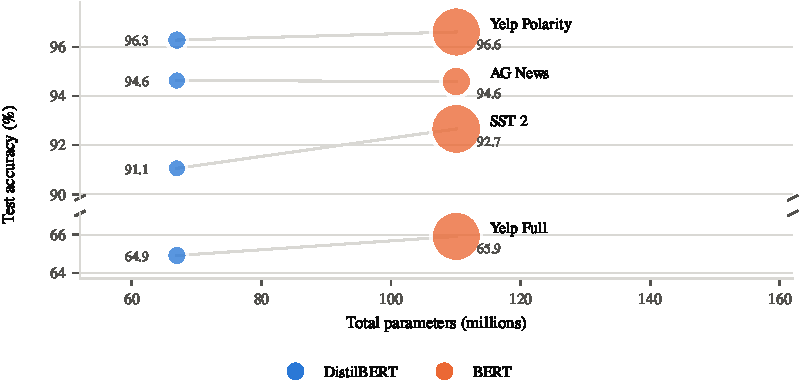
\includegraphics[width=\linewidth]{fig1_params_vs_accuracy_bubble.pdf}
  \caption{Parameters against accuracy. Each line joins the two backbones on one dataset and bubble area is
  single example GPU latency, from \gpuLatencyDistil{} to \gpuLatencyBert{} ms. The lines are close to flat,
  which is this study in one picture.}
  \label{fig:bubble}
\end{figure}

\paragraph{Main comparison.}
Table \ref{tab:main} gives the four performance metrics and Figure \ref{fig:bubble} the required parameter
against accuracy view. The gap averages \meanAccGap{} accuracy points in favour of BERT but is far from
uniform, spanning \minAccGap{} points on \minGapDataset{} to \maxAccGap{} on \maxGapDataset{}: BERT is
clearly ahead on \bertWins{} of the \nDatasets{} datasets and level on the other \distilTiesOrWins{}. Where
a task is close to saturated the two models are indistinguishable, and depth only pays on the harder,
finer grained label set.

\begin{table}[t]
\centering
\footnotesize
\caption{Performance of both backbones with the identical baseline classifier. Precision, recall and F1 are macro averaged.}
\label{tab:main}
\begin{tabular}{llrrrr}
\toprule
Dataset & Model & Accuracy & Precision & Recall & F1 \\
\midrule
AG News & DistilBERT & 94.63 & 94.66 & 94.63 & 94.63 \\
AG News & BERT & 94.59 & 94.63 & 94.59 & 94.59 \\
\addlinespace
SST 2 & DistilBERT & 91.06 & 91.08 & 91.04 & 91.05 \\
SST 2 & BERT & 92.66 & 92.71 & 92.63 & 92.65 \\
\addlinespace
Yelp Polarity & DistilBERT & 96.28 & 96.28 & 96.28 & 96.28 \\
Yelp Polarity & BERT & 96.61 & 96.61 & 96.61 & 96.61 \\
\addlinespace
Yelp Full & DistilBERT & 64.91 & 64.86 & 64.89 & 64.86 \\
Yelp Full & BERT & 65.91 & 65.76 & 65.89 & 65.81 \\
\bottomrule
\end{tabular}
\end{table}


\begin{figure}[!tb]
  \centering
  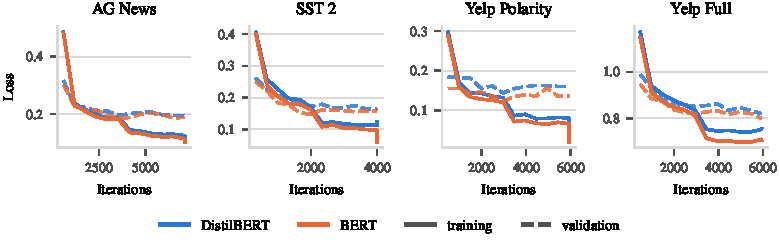
\includegraphics[width=\linewidth]{fig3_loss_curves.pdf}
  \caption{Iterations against training loss (solid) and validation loss (dashed). Both models flatten at
  the same point in the schedule; BERT settles lower.}
  \label{fig:loss}
\end{figure}

\paragraph{How many epochs are needed.}
Two epochs is a choice, so we test it: both backbones are trained on SST 2 and AG News to four epochs, the
top of the published range, scoring the full validation split at every boundary. The best epoch varies
between \epochBestMin{} and \epochBestMax{} across the \epochStudyRuns{} runs with no consistent pattern,
and training past epoch two is worth at most \epochGainOverTwo{} F1 macro points, inside the band we treat
as noise. Two epochs is a defensible stopping point rather than a budget compromise.

\paragraph{Training dynamics.}
Figure \ref{fig:loss} matters beyond bookkeeping: if DistilBERT were merely underfitting, its training loss
would sit high and still be falling at the end. It does not, both models flatten together, so the distance
between the validation curves is a capacity gap and not an optimisation gap.

\paragraph{Efficiency.}
The shape of the saving is worth reading carefully. Halving
the depth should buy a factor of two, and it does exactly that where the device is actually busy:
DistilBERT sustains \throughputDistil{} samples per second at batch 32 against \throughputBert{}, a factor
of \throughputSpeedup{}, and on CPU it needs \cpuLatencyDistil{} ms per example against \cpuLatencyBert{}.
At batch one on the GPU the same models are only \gpuSpeedup{} times apart, \gpuLatencyDistil{} ms against
\gpuLatencyBert{} ms, because a single short sequence leaves the device idle between kernel launches and
the fixed launch cost, not the twelve or six blocks, sets the clock. Peak GPU memory in training falls from
\trainMemBert{} to \trainMemDistil{} GiB, \memReduction{} percent less, and the four runs take
\trainMinutesDistil{} minutes instead of \trainMinutesBert{}.


\section{Analysis}

\paragraph{The classifier head barely matters.}
Across the four head shape variants and the baseline, the full spread in mean F1 macro is \headSpread{}
points (Table \ref{tab:ablation}): narrowing the hidden layer to 128 units,
widening it to 2048, stacking three hidden layers and removing it entirely all land inside that band. After
fine tuning the \texttt{[CLS]} vector is close to linearly separable here, so capacity added on top of it
has nothing left to extract.

\begin{table}[t]\centering\footnotesize
\caption{Pending. The runs behind this table have not finished; src/figures.py writes it as soon as they do.}
\label{tab:ablation}
\begin{tabular}{l}\toprule pending \\ \bottomrule\end{tabular}
\end{table}


\paragraph{Freezing is the axis that matters, and only in its upper half.}
Freezing the whole transformer costs \frozenGap{} F1 macro points against the baseline, more than an order
of magnitude beyond any head shape change. Freezing only the lower three blocks costs \halfFrozenGap{}
points, inside the band that separates the head shapes, while cutting trainable parameters to
\halfFrozenTrainable{}M, \halfFrozenTrainableCut{} percent fewer, and training \halfFrozenSpeedup{} times
faster. Task adaptation therefore lives almost entirely in the upper half of the encoder. This is not a new
result and we do not claim it as one: \citet{kovaleva2019revealing} report that the last two layers of BERT
change most during fine tuning, \citet{merchant2020what} find that fine tuning primarily affects the top
layers, and \citet{lee2019freezing} show that tuning only the final quarter of the layers recovers 90
percent of the quality of tuning all of them. Our runs add that the same holds for a distilled six block
encoder, where there are far fewer layers to give away. The selected variant is \bestVariant{} at
\bestVariantFone{} mean F1 macro, the simplest head in the grid.

\paragraph{The winning variant on BERT.}
Table \ref{tab:best} rebuilds that variant on BERT base. The ordering is unchanged and the gap stays in the
band of the main comparison, so the ablation conclusion belongs to the fine tuning setup rather than to
DistilBERT specifically. Figure \ref{fig:confusion} shows where the remaining errors sit: both models
concentrate them between Business and Sci/Tech, two classes that share vocabulary. The larger model
resolves a few more of those borderline cases but does not fail in different ones, which is the conclusion
the representation analysis below reaches by another route.

\begin{figure}[!tb]
  \centering
  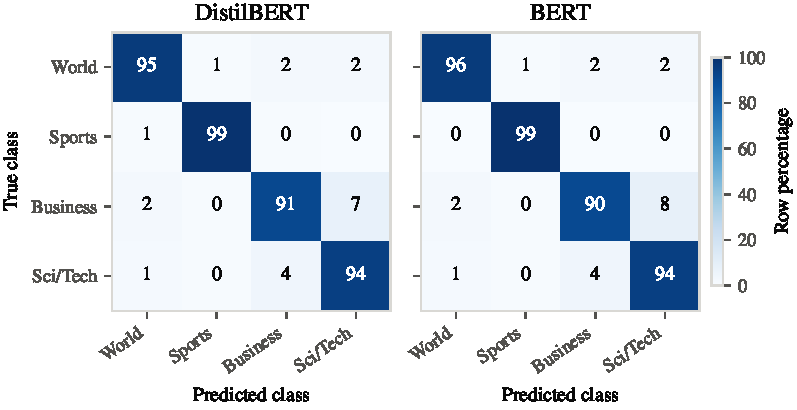
\includegraphics[width=0.72\linewidth]{fig7_confusion_ag_news.pdf}
  \caption{Row normalised confusion matrices on AG News. The two models make the same kind of mistake in
  the same place.}
  \label{fig:confusion}
\end{figure}

\begin{table}[t]
\centering
\scriptsize
\caption{The variant selected by the ablation (G: no hidden layer) on each backbone, with every metric this study records, measured on the same GPU. Within each dataset the better of the two values is in bold, taking lower as better for loss, size, latency, memory and time.}
\label{tab:best}
\begin{tabular}{lrrrr}
\toprule
 & \multicolumn{2}{c}{SST 2} & \multicolumn{2}{c}{AG News} \\
\cmidrule(lr){2-3} \cmidrule(lr){4-5}
 & DistilBERT & BERT & DistilBERT & BERT \\
\midrule
Accuracy (\%) & 91.40 & \textbf{91.97} & \textbf{94.84} & 94.72 \\
Precision, macro (\%) & 91.42 & \textbf{92.01} & \textbf{94.88} & 94.77 \\
Recall, macro (\%) & 91.38 & \textbf{91.95} & \textbf{94.84} & 94.72 \\
F1, macro (\%) & 91.39 & \textbf{91.97} & \textbf{94.85} & 94.73 \\
Test cross entropy & 0.286 & \textbf{0.267} & \textbf{0.168} & \textbf{0.168} \\
Total parameters (M) & \textbf{66.4} & 109.5 & \textbf{66.4} & 109.5 \\
Trainable parameters (M) & \textbf{66.4} & 109.5 & \textbf{66.4} & 109.5 \\
GPU latency, batch 1 (ms) & \textbf{2.23} & 5.12 & \textbf{2.48} & 3.23 \\
CPU latency, batch 1 (ms) & \textbf{27.8} & 53.2 & \textbf{36.4} & 72.2 \\
Throughput, batch 32 (samples/s) & \textbf{2452} & 1218 & \textbf{1220} & 611 \\
Peak GPU memory, training (MiB) & \textbf{1313} & 2302 & \textbf{1706} & 3083 \\
Peak GPU memory, inference (MiB) & \textbf{404} & 569 & \textbf{539} & 706 \\
Training wall clock (min) & \textbf{2.6} & 3.9 & \textbf{4.3} & 7.8 \\
\bottomrule
\end{tabular}
\end{table}


\paragraph{Do the two encoders see language the same way?}
The accuracy gap says how often the models agree on a label, not whether they agree on the geometry
underneath. We compare the geometries with linear centred kernel alignment, CKA
\citep{kornblith2019similarity}. It is the right index here because it is invariant to orthogonal
transformation and isotropic scaling, so a change of basis is not counted as a difference, but not to
arbitrary invertible maps, which is what lets it compare separately trained networks where canonical
correlation analysis cannot. We embed \nWords{} words spanning 20 topics with
each pretrained encoder and compare the two 768 dimensional spaces, matching student block $d$ to teacher
block $2d$, the layer it was initialised from. Alignment is near perfect at
the embeddings (\ckaEmbeddings{}), still high at mid depth (\ckaMid{}) and falls to \ckaTop{} at the top,
so distillation preserved the lower and middle geometry and let the specialised upper layers drift. In the
layer averaged, mean centred space, \wordOverlap{} of the ten nearest neighbours BERT assigns to a word are
also chosen by DistilBERT, and \purityDistil{} percent of DistilBERT neighbours share their query word
topic against \purityBert{} percent for BERT, so the smaller model is marginally tidier here. Fine tuning
then realigns the tops: over AG News test sentences the two fine tuned encoders reach CKA \sentCka{}. An
interactive version ships with the code.

\section{Conclusion}

DistilBERT keeps \accRetention{} percent of the accuracy of BERT base across four datasets while holding
\paramReduction{} percent fewer parameters, reaching \throughputSpeedup{} times its throughput and training
in \memReduction{} percent less GPU memory, so under a latency or memory budget it is the right default on
tasks of this kind. Capacity does not belong in the classifier, where width and depth move F1 macro by at
most \headSpread{} points, but in the upper encoder and only there: freezing all six blocks costs
\frozenGap{} points, freezing the lower three costs \halfFrozenGap{} and trains \halfFrozenSpeedup{} times
faster, and the layerwise alignment agrees, near perfect at the embeddings and \ckaTop{} at the top. Each
run used a single seed, so differences under half a point are noise.

% Tighter reference list: it is not counted in the four page body, so it should
% not spill onto a page of its own for the sake of two entries.
\setlength{\bibsep}{1.5pt plus 0.3ex}
{\small
\bibliographystyle{plainnat}
\bibliography{refs}
}

\end{document}
